\refstepcounter{section}
\section*{Lecture 20: Schwarzschild solution (contd.)}
\addcontentsline{toc}{section}{Lecture 20: Schwarzschild solution (contd.)}
Let us continue our calculation of the geodesic equation. We had already found out the equation for time and the equation for the other coordinates are given as:
\begin{align}
    \vartriangleright \boxed{ \mu = r} \quad &\dv[2]{r}{\tau} + \frac{r_s}{2r^3}(r-r_s)\qty(\dv{t}{\tau})^2 - \frac{r_s}{2r(r-r_s)}\qty(\dv{r}{\tau})^2 -(r-r_s)\qty(\dv{\theta}{\tau}) - (r-r_s)\sin^2\theta\qty(\dv{\phi}{\tau})^2=0\label{eqn:rscs}\\[0.14cm]
\vartriangleright \boxed{ \mu = \theta} \quad &\dv[2]{\theta}{\tau} +\qty(\frac{2}{r})\dv{\theta}{\tau} \dv{r}{\tau}-\sin\theta\cos\theta\qty(\dv{\phi}{\tau})^2=0\label{eqn:tscs}\\[0.14cm]
  \vartriangleright \boxed{ \mu = \phi} \quad &\dv[2]{\phi}{\tau} +\frac{2}{r}\dv{\phi}{\tau}\dv{r}{\tau}+2\cot\theta \dv{\phi}{\tau}\dv{\theta}{\tau}=0\label{eqn:pscs}
\end{align}
Now let us do some analysis based on physical argument. So we want our solution to converge to the Newtonian case in some appropriate limit. We know that the Newtonian solution of motion of planet is confined to a plane since angular momentum is conserved for the problem.\\[0.15cm] Hence, let us also consider a solution restricted to the $\mathrm{x-y}$ plane, that is $\theta=\frac{\pi}{2}$, say for simplicity. Then Eq. \ref{eqn:tscs} is automatically satisfied since the derivatives vanish and $\cos\theta=0$ for this specific angle and hence $\theta=\frac{\pi}{2}$ is a valid solution of Eq. \ref{eqn:tscs}. Let us now see the other equation for this specific case, starting with Eq. \ref{eqn:pscs},
\begin{align*}
    \dv[2]{\phi}{\tau} + \frac{2}{r}\dv{r}{\tau}\dv{\phi}{\tau} = 0 \implies \dv{\tau}\qty(r^2\dv{\phi}{\tau}) = 0 \longrightarrow \boxed{r^2\dot{\phi} = \sfrac{l}{m}}
\end{align*}
where $l$ is some constant. This gives the interpretation of \textit{angular momentum}, with the subtlety that now, the derivative is with respect to the proper time $\tau$. We thus see that the assumption of planar motion directly handed us the conservation of angular momentum here also. \\[0.2cm]
Let us recall a bit about the Newtonian Lagrangian for the motion of the planet. The general Lagrangian in spherical polar coordinates for the Newtonian case is given by:
$$\SL = \frac{1}{2}m\qty(\dot{r}^2+ r^2\dot{\theta}^2+ r^2\sin^2\theta \dot{\phi}^2)- V_N \quad \xrightarrow{\theta=\sfrac{\pi}{2}} \SL =  \frac{1}{2}m\qty(\dot{r}^2+ r^2 \dot{\phi}^2)-V_N$$
where $V_N$ denotes the Newtonian potential and for this problem, $V_N = -\frac{GM}{r}$. We now find the ELEOM from this:
\begin{align*}
    &\dv{t}\qty(\pdv{\SL}{\dot{\phi}}) = \dv{\SL}{\phi} \longrightarrow \dv{t}\qty(mr^2\dot{\phi}) = 0\\
    &\dv{t}\qty(\pdv{\SL}{\dot{r}}) = \dv{\SL}{r} \longrightarrow \ddot{r} = \pdv{r}\qty(\frac{1}{2}mr^2\dot{\phi}^2 -V_N) = \pdv{r}\qty(\frac{l^2}{2mr^2} )
\end{align*}
Thus, we see that the body `feels' two potentials and we can thus define an \textit{effective potential} as $V^{\mathrm{eff}}_{\textrm{N}}$ as:
\begin{align}
    \boxed{V^{\mathrm{eff}}_{\textrm{N}} := V_N + \frac{l^2}{2mr^2} = -\frac{GM}{r} + \frac{l^2}{2mr^2}}\label{eqn:veffn}
\end{align}
Now, let us come back to Eq. \ref{eqn:rscs} and write it in the form below:
\begin{align}
    \dv[2]{r}{\tau} + \frac{r_s}{2r^2} \qty[\qty(\frac{r-r_s}{r}) \qty(\dv{t}{\tau})^2 - \qty(\frac{r}{r-r_s}) \qty(\dv{r}{\tau})^2] - (r-r_s)\frac{l^2}{m^2r^4} =0
\end{align}
Now consider the metric in Eq. \ref{eqn:metric} in the case when $\theta=\sfrac{\pi}{2}$,
$$ds^2 = -\qty(1- \frac{r_s}{r})\dd t^2 + \qty(1- \frac{r_s}{r})^{-1} \dd r^2 +r^2 \dd \phi^2$$
Also, recall that in natural units, $\dd s^2 = -\dd \tau^2$ and rearranging the equation gives us:
$$1+ r^2 \qty(\dv{\phi}{\tau})^2 = \frac{r- r_s}{r}\qty(\dv{t}{\tau})^2 - \frac{r}{r-r_s}\qty(\dv{r}{\tau})^2$$
Substituting this in Eq. \ref{eqn:rscs} we get:
$$\dv[2]{r}{\tau}+ \frac{r_s}{2r^2}\qty(1+r^2 \times \frac{l^2}{m^2r^4})-(r-r_s)\frac{l^2}{m^2r^4} =0\implies \boxed{\dv[2]{r}{\tau} = \frac{l^2}{m^2r^3} - \frac{3r_sl^2}{2m^2r^4} - \frac{r_s}{2r^2}}$$
From this, we can define an effective potential as $\sfrac{\dd^2 r}{\dd \tau^2} = - \sfrac{\partial V^{\mathrm{eff}}_{\textrm{GR}}}{\partial r}$ where, 
\begin{align}\label{eqn:veffgr}
    \boxed{{V^{\mathrm{eff}}_{\textrm{GR}}} = -\frac{r_s}{2r} + \frac{l^2}{2m^2 r^2} \qty(1 - \frac{r_s}{r})}
\end{align}
We have to somehow reconcile Eq. \ref{eqn:veffgr} and Eq. \ref{eqn:veffn} in an appropriate limit. These look very similar and we can do an identification:
$$r_s = 2GM$$
Also note that if, $\sfrac{r_s}{r}\ll 1$ then the second term of \ref{eqn:veffgr} coincides with the second term of Eq. \ref{eqn:veffn}. Hence we conclude that $r\ll r_s$ determines the Newtonian limit. We thus obtain a characteristic length scale $r_s$ which we term as the \textit{Schwarzschild radius}. For a massive object, the solution metric of the Einstein equation becomes:
$$\boxed{ds^2 = - \qty(1- \frac{2GM}{r})\ \dd t^2 + \qty(1 - \frac{2GM}{r})^{-1}\ \dd r^2 + r^2(\dd \theta^2 + \sin^2\theta \ \dd\phi^2)}$$
And the radial equation becomes in terms of the Schwarzschild radius as:
\begin{equation}\label{eqn:radial}
    \boxed{\dv[2]{r}{\tau} = \frac{l^2}{m^2r^3} - \frac{3GMl^2}{m^2r^4} - \frac{GM}{r^2}}
\end{equation}
\subsection{GPS and relativity! }
GPS (global positioning system) works on the process of \textit{trilateration} where different satellites orbiting the Earth convey their position to the receiver (and thus for each satellite we can draw a sphere of radius equal to the distance between the receiver and the satellite) and based on the intersection of these spheres, we can pinpoint our location. 
\begin{figure}[H]
    \centering 
    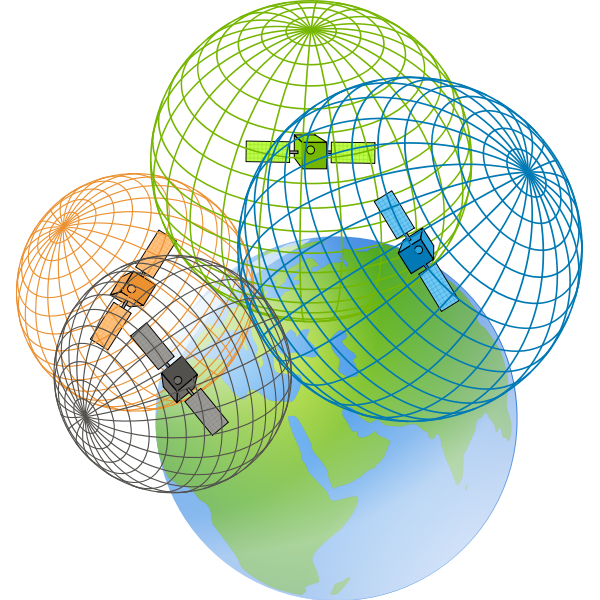
\includegraphics[scale=0.25]{pics/gps.png}
    \caption{The process of trilateration}
\end{figure}
\noindent
The satellites transmit the time of transmission of the radio signal and from there, we indirectly calculate the distance by the difference of the time of transmission and the time of receipt. However, due to the effects of special and general relativity, correction is needed as the clock on Earth and the satellite do not run at the same rate. \footnote{Due to SR, clock in the satellite run slower ($\sim 7 \mu s$/day) while due to GR, clock in a lower gravitational field move faster ($\sim 45 \mu s$/day), thus there is an error offset of $+38\mu s$/day which is corrected by the GPS.}